% CVPR 2023 Paper Template
% based on the CVPR template provided by Ming-Ming Cheng (https://github.com/MCG-NKU/CVPR_Template)
% modified and extended by Stefan Roth (stefan.roth@NOSPAMtu-darmstadt.de)

\documentclass[10pt,twocolumn,letterpaper]{article}

%%%%%%%%% PAPER TYPE  - PLEASE UPDATE FOR FINAL VERSION
\usepackage{cvpr}      % To produce the REVIEW version


% Include other packages here, before hyperref.
\usepackage{graphicx}
\usepackage{amsmath}
\usepackage{amssymb}
\usepackage{booktabs}

% It is strongly recommended to use hyperref, especially for the review version.
% hyperref with option pagebackref eases the reviewers' job.
% Please disable hyperref *only* if you encounter grave issues, e.g. with the
% file validation for the camera-ready version.
%
% If you comment hyperref and then uncomment it, you should delete
% ReviewTempalte.aux before re-running LaTeX.
% (Or just hit 'q' on the first LaTeX run, let it finish, and you
%  should be clear).
\usepackage[pagebackref,breaklinks,colorlinks]{hyperref}


% Support for easy cross-referencing
\usepackage[capitalize]{cleveref}
\crefname{section}{Sec.}{Secs.}
\Crefname{section}{Section}{Sections}
\Crefname{table}{Table}{Tables}
\crefname{table}{Tab.}{Tabs.}


%%%%%%%%% PAPER ID  - PLEASE UPDATE
\def\cvprPaperID{*****} % *** Enter the CVPR Paper ID here
\def\confName{CVPR}
\def\confYear{2023}


\begin{document}

%%%%%%%%% TITLE - PLEASE UPDATE
\title{Team \#16: From Strings to Sequences --- Classifying and Generating Music from Acoustic Guitar Notes}

\author{
Camilo Martínez\\
7057573\\
\and
Dhimitrios Duka\\
7059153\\
\and
Honglu Ma\\
7055053\\
}
\maketitle

%%%%%%%%% BODY TEXT
\section{Task and Motivation}
Automatic cord recognition (ACR) consists of recognizing the chords being played in a music piece. This information is quite valuable since it can later be used for music analysis, music transcription, or even fixing corrupted musical performances. ACR was first introduced in 1999 by \cite{takuya1999realtime} where the author utilized lisp music to perform chord recognition at the signal level. Since then, many signal-level based approaches have been introduced. However, these methods proved to be quite challenging and not very accurate. 

With the rise of deep learning, and especially computer vision, many researches started to tackle this problem from a different perspective. They started to use spectrogram-based feature extraction methods to extract the features of the audio signal \cite{boulanger2013audio, korzeniowski2016feature, stark2009real}. However, despi


Task statement and definitions

Motivation: Why do we need to explore this task?

\textbf{Related work: How do existing papers solve this task or similar tasks (should include relevant citations)?}

For the task of fretboard detection, Y. Kristian et al. \cite[2024]{Kristian_Zaman_Tenoyo_Jodhinata_2024} employed a Single Shot Detection (SSD) model undergirded by a MobileNetV2 base model, pre-trained on the Ego-Hand dataset. The subsystem processes the input image or video frame using a Deep Convolutional Neural Network (DCNN) model. The model generates coordinates for bounding boxes that outline thefretboard.

\textbf{Challenge: What are the major challenges that have not been solved in this task?}

\cite{Kristian_Zaman_Tenoyo_Jodhinata_2024}
\cite{du2023conditional}

\section{Goals}

\begin{figure*}[h]
    \centering
    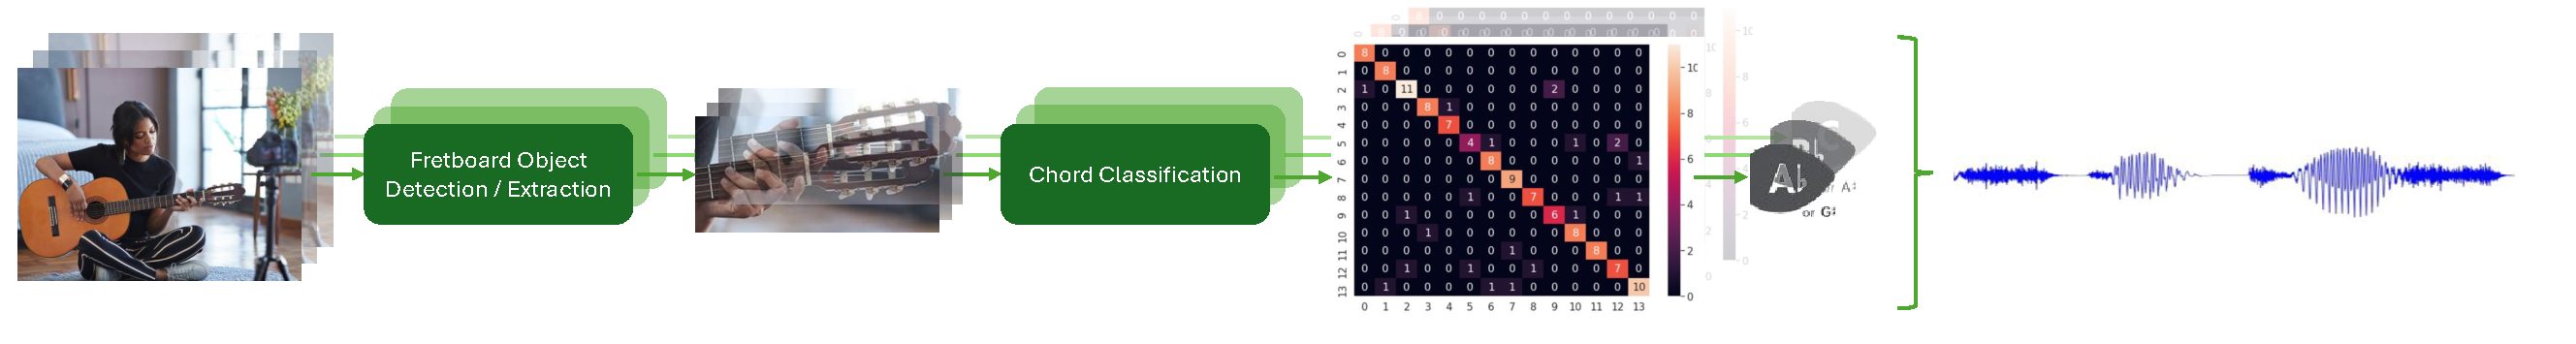
\includegraphics[width=\textwidth]{images/task-diagram.pdf}
    \caption{Overview of the Model, showcasing the 2 most important tasks: 
    Fretboard Detection and Chord Classification, done for each frame of an input video. Image taken from \textit{Getty Stock Images}, confusion matrix image taken from \cite{Kristian_Zaman_Tenoyo_Jodhinata_2024}.}
    \label{fig:model-diagram}
\end{figure*}

\textbf{What challenges do you aim to address in this task?}
\cref{fig:model-diagram} illustrates a bird's eye view of our model architecture. Essentially, we aim to address the following 3 problems: 
\begin{enumerate}
    \item Fretboard Detection: Given an image or video frame, detect the fretboard of the guitar.
    \item Chord Classification: Given an image or video frame, classify the chord being played.
    \item Seamless Audio Generation: Given the chords being played, generate the audio of the music piece.
\end{enumerate}
the problem of chord recognition in a video. This is a challenging task since the video contains both audio and visual information. We aim to use both of these information to improve the accuracy of the chord recognition.


\textbf{What do you want to have completed by the mid-term? E.g., code for the task, data collection, results for baselines, etc.}




\section{Methods}

What models/frameworks do you use to solve the challenges?

Why can the proposed method / analysis solve your problem?

What are the main differences between your method and existing methods (if applicable)?

What is the required computational budget for the training/analysis? (E.g. are you planning on using pretrained backbones?)

\section{Datasets}

What datasets are you going to use/collect and why?


\subsection{Fretboard Detection}
This one has both: \cite{guitar-chords-daewp_dataset}. 
Only fretboard: \cite{guitar-ppfil_dataset}, \cite{done-npcll_dataset}.

\subsection{Chord Recognition}
For chord recognition: \cite{guitar-chord-tvon8_dataset}, \cite{guitar-chord-bounding-box_dataset}, \cite{guitar-chord-handshape_dataset}.

\subsection{Seamless Audio Generation}
\emph{GuitarSet}, a dataset that provides high quality acoustic guitar recordings alongside time-aligned annotations including fret positions, chords, among others \cite{Xi2018}.

\section{Evaluation}

How is your method going to be evaluated?

What metrics are suitable?

Do you need to define your own metric for evaluation?

\clearpage 

%%%%%%%%% REFERENCES
{\small
\bibliographystyle{ieee_fullname}
\bibliography{references}
}

\end{document}
